%%% Hlavní soubor. Zde se definují základní parametry a odkazuje se na ostatní části. %%%

%% Verze pro jednostranný tisk:
% Okraje: levý 40mm, pravý 25mm, horní a dolní 25mm
% (ale pozor, LaTeX si sám přidává 1in)
\documentclass[12pt,a4paper]{report}
\setlength\textwidth{145mm}
\setlength\textheight{247mm}
\setlength\oddsidemargin{15mm}
\setlength\evensidemargin{15mm}
\setlength\topmargin{0mm}
\setlength\headsep{0mm}
\setlength\headheight{0mm}
% \openright zařídí, aby následující text začínal na pravé straně knihy
\let\openright=\clearpage

%% Pokud tiskneme oboustranně:
% \documentclass[12pt,a4paper,twoside,openright]{report}
% \setlength\textwidth{145mm}
% \setlength\textheight{247mm}
% \setlength\oddsidemargin{14.2mm}
% \setlength\evensidemargin{0mm}
% \setlength\topmargin{0mm}
% \setlength\headsep{0mm}
% \setlength\headheight{0mm}
% \let\openright=\cleardoublepage

%% Vytváříme PDF/A-2u
\usepackage[a-2u]{pdfx}

%% Přepneme na českou sazbu a fonty Latin Modern
\usepackage[czech]{babel}
\usepackage{lmodern}
\usepackage[T1]{fontenc}
\usepackage{textcomp}

%% Použité kódování znaků: obvykle latin2, cp1250 nebo utf8:
\usepackage[utf8]{inputenc}

%%% Další užitečné balíčky (jsou součástí běžných distribucí LaTeXu)
\usepackage{amsmath}        % rozšíření pro sazbu matematiky
\usepackage{amsfonts}       % matematické fonty
\usepackage{amsthm}         % sazba vět, definic apod.
\usepackage{bbding}         % balíček s nejrůznějšími symboly
			    % (čtverečky, hvězdičky, tužtičky, nůžtičky, ...)
\usepackage{bm}             % tučné symboly (příkaz \bm)
\usepackage{graphicx}       % vkládání obrázků
\usepackage{fancyvrb}       % vylepšené prostředí pro strojové písmo
\usepackage{indentfirst}    % zavede odsazení 1. odstavce kapitoly
\usepackage{natbib}         % zajištuje možnost odkazovat na literaturu
			    % stylem AUTOR (ROK), resp. AUTOR [ČÍSLO]
\usepackage[nottoc]{tocbibind} % zajistí přidání seznamu literatury,
                            % obrázků a tabulek do obsahu
\usepackage{icomma}         % inteligetní čárka v matematickém módu
\usepackage{dcolumn}        % lepší zarovnání sloupců v tabulkách
\usepackage{booktabs}       % lepší vodorovné linky v tabulkách
\usepackage{paralist}       % lepší enumerate a itemize
\usepackage{xcolor}         % barevná sazba
\usepackage{listings}		% code higlighting

\graphicspath{ {../img/} }

\definecolor{bluekeywords}{rgb}{0.13,0.13,1}
\definecolor{greencomments}{rgb}{0,0.5,0}
\definecolor{redstrings}{rgb}{0.9,0,0}


%%% Údaje o práci

% Název práce v jazyce práce (přesně podle zadání)
\def\NazevPrace{Aplikace pro správu výukových kurzů}

% Název práce v angličtině
\def\NazevPraceEN{Application for Educational Courses Management}

% Jméno autora
\def\AutorPrace{Vojtěch Lengál}

% Rok odevzdání
\def\RokOdevzdani{2021}

% Název katedry nebo ústavu, kde byla práce oficiálně zadána
% (dle Organizační struktury MFF UK, případně plný název pracoviště mimo MFF)
\def\Katedra{Katedra distribuovaných a spolehlivých systémů}
\def\KatedraEN{Department of Distributed and Dependable Systems}

% Jedná se o katedru (department) nebo o ústav (institute)?
\def\TypPracoviste{Katedra}
\def\TypPracovisteEN{Department}

% Vedoucí práce: Jméno a příjmení s~tituly
\def\Vedouci{doc. RNDr. Jan Kofroň, Ph.D.}

% Pracoviště vedoucího (opět dle Organizační struktury MFF)
\def\KatedraVedouciho{Katedra distribuovaných a spolehlivých systémů}
\def\KatedraVedoucihoEN{Department of Distributed and Dependable Systems}

% Studijní program a obor
\def\StudijniProgram{Informatika}
\def\StudijniObor{Softwarové a datové inženýrství}

% Nepovinné poděkování (vedoucímu práce, konzultantovi, tomu, kdo
% zapůjčil software, literaturu apod.)
\def\Podekovani{%
Tímto bych chtěl poděkovat vedoucímu práce doc. RNDr. Janu Kofroňovi, Ph.D. za jeho rady a připomínky.
}

% Abstrakt (doporučený rozsah cca 80-200 slov; nejedná se o zadání práce)
\def\Abstrakt{%
Cílem práce je vytvořit webovou aplikaci pro správu různých typů výukových kurzů, jako například vysokoškolské přednášky a cvičení, předměty na základní či střední škole nebo také libovolný zájmový kurz. Program bude poskytovat rozhraní jak pro správce – učitele, tak pro uživatele – studenty. Bude umožňovat vytváření a správu kurzů. Správci kurzu budou moci měnit jeho obsah (přidávat, odebírat materiály, apod.) a zakládat nové úkoly a testy, které budou uživatelé následně vyplňovat. Otázky s nabídkou odpovědí bude systém vyhodnocovat automaticky, zbytek bude správce kurzu hodnotit ručně. Uživatel si pak bude moci v daném kurzu prohlédnout všechny známky, a také opravené testy a úkoly.
}
\def\AbstraktEN{%
Abstract.
}

% 3 až 5 klíčových slov (doporučeno), každé uzavřeno ve složených závorkách
\def\KlicovaSlova{%
{klíčová} {slova}
}
\def\KlicovaSlovaEN{%
{key} {words}
}

%% Balíček hyperref, kterým jdou vyrábět klikací odkazy v PDF,
%% ale hlavně ho používáme k uložení metadat do PDF (včetně obsahu).
%% Většinu nastavítek přednastaví balíček pdfx.
\hypersetup{unicode}
\hypersetup{breaklinks=true}

%% Definice různých užitečných maker (viz popis uvnitř souboru)
%%% Tento soubor obsahuje definice různých užitečných maker a prostředí %%%
%%% Další makra připisujte sem, ať nepřekáží v ostatních souborech.     %%%

%%% Drobné úpravy stylu

% Tato makra přesvědčují mírně ošklivým trikem LaTeX, aby hlavičky kapitol
% sázel příčetněji a nevynechával nad nimi spoustu místa. Směle ignorujte.
\makeatletter
\def\@makechapterhead#1{
  {\parindent \z@ \raggedright \normalfont
   \Huge\bfseries \thechapter. #1
   \par\nobreak
   \vskip 20\p@
}}
\def\@makeschapterhead#1{
  {\parindent \z@ \raggedright \normalfont
   \Huge\bfseries #1
   \par\nobreak
   \vskip 20\p@
}}
\makeatother

% Toto makro definuje kapitolu, která není očíslovaná, ale je uvedena v obsahu.
\def\chapwithtoc#1{
\chapter*{#1}
\addcontentsline{toc}{chapter}{#1}
}

% Trochu volnější nastavení dělení slov, než je default.
\lefthyphenmin=2
\righthyphenmin=2

% Zapne černé "slimáky" na koncích řádků, které přetekly, abychom si
% jich lépe všimli.
\overfullrule=1mm

%%% Makra pro definice, věty, tvrzení, příklady, ... (vyžaduje baliček amsthm)

\theoremstyle{plain}
\newtheorem{veta}{Věta}
\newtheorem{lemma}[veta]{Lemma}
\newtheorem{tvrz}[veta]{Tvrzení}

\theoremstyle{plain}
\newtheorem{definice}{Definice}

\theoremstyle{remark}
\newtheorem*{dusl}{Důsledek}
\newtheorem*{pozn}{Poznámka}
\newtheorem*{prikl}{Příklad}

%%% Prostředí pro důkazy

\newenvironment{dukaz}{
  \par\medskip\noindent
  \textit{Důkaz}.
}{
\newline
\rightline{$\qedsymbol$}
}

%%% Prostředí pro sazbu kódu, případně vstupu/výstupu počítačových
%%% programů. (Vyžaduje balíček fancyvrb -- fancy verbatim.)

\DefineVerbatimEnvironment{code}{Verbatim}{fontsize=\small, frame=single}

%%% Prostor reálných, resp. přirozených čísel
\newcommand{\R}{\mathbb{R}}
\newcommand{\N}{\mathbb{N}}

%%% Užitečné operátory pro statistiku a pravděpodobnost
\DeclareMathOperator{\pr}{\textsf{P}}
\DeclareMathOperator{\E}{\textsf{E}\,}
\DeclareMathOperator{\var}{\textrm{var}}
\DeclareMathOperator{\sd}{\textrm{sd}}

%%% Příkaz pro transpozici vektoru/matice
\newcommand{\T}[1]{#1^\top}

%%% Vychytávky pro matematiku
\newcommand{\goto}{\rightarrow}
\newcommand{\gotop}{\stackrel{P}{\longrightarrow}}
\newcommand{\maon}[1]{o(n^{#1})}
\newcommand{\abs}[1]{\left|{#1}\right|}
\newcommand{\dint}{\int_0^\tau\!\!\int_0^\tau}
\newcommand{\isqr}[1]{\frac{1}{\sqrt{#1}}}

%%% Vychytávky pro tabulky
\newcommand{\pulrad}[1]{\raisebox{1.5ex}[0pt]{#1}}
\newcommand{\mc}[1]{\multicolumn{1}{c}{#1}}


\lstdefinestyle{sharpc}{language=[Sharp]C,
	showspaces=false,
	showtabs=false,
	breaklines=true,
	showstringspaces=false,
	breakatwhitespace=true,
	escapeinside={(*@}{@*)},
	commentstyle=\color{greencomments},
	keywordstyle=\color{bluekeywords}\bfseries,
	stringstyle=\color{redstrings},
	basicstyle=\small\ttfamily,
	tabsize=4
}

\lstdefinelanguage{Typescript}{
	keywords={break, case, catch, continue, debugger, default, delete, do, else, finally, for, function, if, in, instanceof, new, return, switch, this, throw, try, typeof, var, void, while, with, private, protected, public, abstract, let, const, readonly, constructor, class, export, boolean, string, number, throw, implements, import, this, super, static},
	identifierstyle=\color{black},
	comment=[l]{//},
	morecomment=[s]{/*}{*/},
	morestring=[b]',
	morestring=[b]",
	morestring=[b]`
}

\lstdefinestyle{typescript}{language=Typescript,
	showspaces=false,
	showtabs=false,
	breaklines=true,
	showstringspaces=false,
	breakatwhitespace=true,
	escapeinside={(*@}{@*)},
	commentstyle=\color{greencomments},
	keywordstyle=\color{bluekeywords}\bfseries,
	stringstyle=\color{redstrings},
	basicstyle=\small\ttfamily,
	tabsize=4
}

\lstdefinestyle{html}{language=HTML,
	showspaces=false,
	showtabs=false,
	breaklines=true,
	showstringspaces=false,
	breakatwhitespace=true,
	commentstyle=\color{greencomments},
	keywordstyle=\color{bluekeywords}\bfseries,
	stringstyle=\color{redstrings},
	basicstyle=\small\ttfamily,
	tabsize=4
}

\lstset{style=sharpc}

%% Titulní strana a různé povinné informační strany
\begin{document}
%%% Titulní strana práce a další povinné informační strany

%%% Titulní strana práce

\pagestyle{empty}
\hypersetup{pageanchor=false}

\begin{center}

\centerline{\mbox{
\includegraphics[width=166mm]{../img/logo-cs.pdf}}}

\vspace{-8mm}
\vfill

{\bf\Large BAKALÁŘSKÁ PRÁCE}

\vfill

{\LARGE\AutorPrace}

\vspace{15mm}

{\LARGE\bfseries\NazevPrace}

\vfill

\Katedra

\vfill

{
\centerline{\vbox{\halign{\hbox to 0.45\hsize{\hfil #}&\hskip 0.5em\parbox[t]{0.45\hsize}{\raggedright #}\cr
Vedoucí bakalářské práce:&\Vedouci \cr
\noalign{\vspace{2mm}}
Studijní program:&\StudijniProgram \cr
\noalign{\vspace{2mm}}
Studijní obor:&\StudijniObor \cr
}}}}

\vfill

% Zde doplňte rok
Praha \RokOdevzdani

\end{center}

\newpage

%%% Následuje vevázaný list -- kopie podepsaného "Zadání bakalářské práce".
%%% Toto zadání NENÍ součástí elektronické verze práce, nescanovat.

%%% Strana s čestným prohlášením k bakalářské práci

\openright
\hypersetup{pageanchor=true}
\pagestyle{plain}
\pagenumbering{roman}
\vglue 0pt plus 1fill

\noindent
Prohlašuji, že jsem tuto bakalářskou práci vypracoval(a) samostatně a výhradně
s~použitím citovaných pramenů, literatury a dalších odborných zdrojů.
Tato práce nebyla využita k získání jiného nebo stejného titulu.

\medskip\noindent
Beru na~vědomí, že se na moji práci vztahují práva a povinnosti vyplývající
ze zákona č. 121/2000 Sb., autorského zákona v~platném znění, zejména skutečnost,
že Univerzita Karlova má právo na~uzavření licenční smlouvy o~užití této
práce jako školního díla podle §60 odst. 1 autorského zákona.

\vspace{10mm}

\hbox{\hbox to 0.5\hsize{%
V \hbox to 6em{\dotfill} dne \hbox to 6em{\dotfill}
\hss}\hbox to 0.5\hsize{\dotfill\quad}}
\smallskip
\hbox{\hbox to 0.5\hsize{}\hbox to 0.5\hsize{\hfil Podpis autora\hfil}}

\vspace{20mm}
\newpage

%%% Poděkování

\openright

\noindent
\Podekovani

\newpage

%%% Povinná informační strana bakalářské práce

\openright

\vbox to 0.5\vsize{
\setlength\parindent{0mm}
\setlength\parskip{5mm}

Název práce:
\NazevPrace

Autor:
\AutorPrace

\TypPracoviste:
\Katedra

Vedoucí bakalářské práce:
\Vedouci, \KatedraVedouciho

Abstrakt:
\Abstrakt

Klíčová slova:
\KlicovaSlova

\vss}\nobreak\vbox to 0.49\vsize{
\setlength\parindent{0mm}
\setlength\parskip{5mm}

Title:
\NazevPraceEN

Author:
\AutorPrace

\TypPracovisteEN:
\KatedraEN

Supervisor:
\Vedouci, \KatedraVedoucihoEN

Abstract:
\AbstraktEN

Keywords:
\KlicovaSlovaEN

\vss}

\newpage

\openright
\pagestyle{plain}
\pagenumbering{arabic}
\setcounter{page}{1}


%%% Strana s automaticky generovaným obsahem bakalářské práce

\tableofcontents

%%% Jednotlivé kapitoly práce jsou pro přehlednost uloženy v samostatných souborech
\chapter{Úvod}


Cílem je vytvořit webovou aplikaci na správu různých typů výukových kurzů. Pod kurzem si můžeme představit např. přednášku/cvičení na vysoké škole nebo předmět na základní popř. střední škole. Studenti budou moci prostřednictvím tohoto systému odevzdávat a vypracovávat testy a úkoly, které jim následně správce kurzu opraví. 
Aplikace bude ale také umožňovat vytvoření kurzů bez hodnocení (tzv. non-graded courses), ty mohou být vhodné např. pro různé zájmové kurzy, kde úkoly ani testy nedávají smysl. 
Alternativy jsou např. aplikace Bakaláři a Moodle. Na rozdíl od těchto programů nebude výsledná aplikace tak úzce zaměřená pro školy (bude ji možné snadno použít i např. na jazykové, zájmové kurzy, apod.).
Program plánuju vyvíjet jako open-source, zdrojový kód bude ve veřejném repozitáři na Githubu.

(převzato ze specifikace ročníkové práce)
%%% Fiktivní kapitola s ukázkami sazby

\chapter{Popis a analýza použitých technologií}

V této kapitole se nachází popis technologií, použitých při vývoji aplikace.

Program je ve formě single-page webové aplikace, což je v dnešní době velmi rozšířený typ webových aplikací.

Každá webová aplikace je typicky rozdělená na dvě části: serverovou a klientskou část. Serverová část aplikace běží na serveru a často má na starosti komunikaci s databází a vnitřní logiku aplikace. Klientská část běží naopak v prohlížeči uživatele a často bývá naprogramovaná v jazyce JavaScript. 

Klasické webové aplikace mají typicky velkou většinu kódu v serverové části. Při dotazu na danou URL server požadavek zpracuje, a vrátí uživateli vygenerované HTML.

Single-page aplikace přesouvají část kódu do klientské části a dotazy na server, který typicky funguje jako API, probíhají ve většině případů asynchronně na pozadí.
Server vrací data ve formátu JSON, jež jsou následně zpracovány klientem. Oproti klasickým webovým aplikacím tedy není potřeba při dotazu na data stránku znovu načítat.
Single-page aplikace nám umožňují oddělení serverové a klientské části, každá část může být napsána v jiném programovacím jazyce.

Velkou výhodou webových aplikací je jejich přenositelnost, jelikož klientská část typicky může běžet v libovolném prohlížeči.
Další výhodou je jednoduchosti použití, uživatel nemusí program stahovat ani instalovat, stačí pouze mít webový prohlížeč.

V následujících podkapitolách se nachází popis použitých technologií a uvedení případných alternativ.

\section{Serverová část}

\subsection{Jazyk C\#}
C\# je objektově orientovaný, staticky typovaný programovací jazyk, vyvinutý firmou Microsoft.
C\# podporuje koncepty zapouzdření, dědičnosti a polymorfismu. Programy v jazyce C\# běží na platformě .NET. 
Při kompilaci C\# programu je zdrojový kód nejprve zkompilován do mezikódu zvaného CIL. 
Po spuštění programu pak modul CLR, který je součástí platformy .NET, provede JIT (just-in-time) kompilaci IL kódu do strojových instrukcí počítače.
Jazyk C\# lze využít k tvorbě konzolových aplikací, webových aplikací a stránek, formulářových aplikací ve Windows, softwaru pro mobilní zařízení, apod. 
\cite{CSharpDocs}

Jazyk C\# využíváme v serverové části aplikace. Používáme platformu .NET Core verze 3.1 a jazyk C\# verze 8.0.

\subsection{ASP .NET Core}
ASP.NET Core je open source framework, který slouží k vývoji webových aplikací na platformě .NET Core. Aplikace je možné psát v libovolném jazyce, který běží na platformě .NET Core (například v jazyce C\#). Jedná se o novější alternativu k frameworku ASP .NET. Součástí frameworku je mimo jiné webový server Kestrel a vestavěný IoC kontejner.
\cite{AspNetCoreDocs}

V aplikaci používáme framework ASP .NET Core verze 3.1 v projektu API. Tento projekt funguje jako REST API a slouží k obsluze HTTP požadavků.

\subsection{Entity Framework Core}
Entity Framework Core je ORM framework. Objektově relační mapování je technika, která nám umožňuje objektově pracovat s daty v relační databázi. Framework reprezentuje databázové tabulky pomocí kolekcí, jednotlivé objekty v kolekci pak představují řádky v dané tabulce. Při práci s databází pak vůbec nepoužíváme jazyk SQL, pouze pracujeme s objekty a kolekcemi.
\cite{EfCoreDocs}

Tento framework využíváme v projektu Data, ve kterém se nachází objekty reprezentující databázové entity, a v projektu \textit{Services}, který obsahuje služby pro komunikaci s databází.

\subsection{xUnit.net}
xUnit.net je framework, který slouží k testování aplikací na platformě .NET. Nejčastěji se používá k unit a integračním testům. 
\cite{xUnitDocs}

V aplikaci tento používáme xUnit.net v projektu TestEvaluation.Tests, který obsahuje unit testy tříd z projektu TestEvaluation.

\subsection{Alternativy}

K vývoji serverové části aplikace můžeme použít velké množství jiných technologií, jelikož většina populárních programovacích jazyků nabízí nějakou knihovnu, příp. framework pro tvorbu webových aplikací.  Jako příklad můžeme uvést jazyk Java v kombinaci s frameworkem Spring, PHP nebo Python s knihovnou Flask. 

Jazyk C\# s použitím frameworku ASP .NET Core jsem zvolil hlavně z toho důvodu, že se jedná o moderní staticky typovaný jazyk, který považuji za nejlepší volbu z výše uvedených. S vývojem v tomto jazyce mám také nejvíce zkušeností. 

Pro práci s databází existuje v jazyce C\# velké množství knihoven a frameworků. Kromě již zmíněného frameworku Entity Framework Core můžeme uvést také knihovnu ADO.NET, micro ORM Dapper a framework NHibernate. 
Tyto technologie se můžou lišit podle míry abstrakce nad databází, např. při použití frameworku Dapper se dotazujeme pomocí klasického SQL, naopak Entity Framework Core nám umožňuje s tabulkami pracovat stejně jako s kolekcemi.

Entity Framework Core je v současnosti pravděpodobně nejpoužívanější z těchto technologií, a umožňuje nám pracovat s databází velmi pohodlně, z tohoto důvodu jsem jej tedy v aplikaci použil. 

\section{Klientská část}

\subsection{Jazyk TypeScript}
TypeScript je programovací jazyk vyvinutý firmou Microsoft. Jedná se o nadstavbu jazyka JavaScript, oba jazyky tedy používají stejnou syntaxi. Kód v jazyce TypeScript se kompiluje do JavaScriptu.
Oproti jazyku JavaScript používá statické typování a umožňuje používat třídy, rozhraní a další konstrukce z OOP. 
\cite{TypescriptDocs}

Téměř celá klientská část aplikace (kromě HTML šablon a CSS stylů) je napsána v jazyce TypeScript.

\subsection{Angular}
Angular je frontend framework pro tvorbu single-page webových aplikací. Framework používá jazyk TypeScript a jeho architektura je založená na komponentách.
Komponenty jsou jednotky kódu, ze kterých se skládá UI aplikace. Každá komponenta obsahuje TypeScript třídu označenou dekorátorem \textit{@Component()}, HTML šablonu, a případně i soubor s CSS styly. 
Součástí frameworku je i vestavěný HTTP klient pro snadnější komunikaci pomocí HTTP, router sloužící k navigaci mezi stránkami a velké množství dalších knihoven. Angular nám umožňuje používat obousměrný data binding.
\cite{AngularDocs}

Tento framework využíváme v klientské části aplikace, celá klientská část programu je Angular projekt.

\subsection{Bootstrap}
Bootstrap je CSS framework, který se používá k designu webových stránek.
Umožňuje jednoduše vytvářet responzivní layout a obsahuje velké množství definovaných CSS stylů, které lze použít ke stylování HTML elementů.
\cite{BootstrapDocs}

Bootstrap hojně používáme ke stylování HTML elementů v šablonách Angular komponent.

\subsection{Alternativy}
K vývoji klientské části aplikace se nejčastěji používá jazyk JavaScript, případně jeho nadstavba TypeScript. Mezi nejpoužívanější frameworky patří v současnosti Angular, React a Vue.js. 
Poměrně novou možností je technologie WebAssembly, zde můžeme uvést například framework Blazor, jež nám umožňuje programovat klientskou část aplikace v jazyce C\#.

Tyto technologie velmi zjednodušují tvorbu moderních a přívětivých uživatelských rozhraní. 
Ve většině případů tyto frameworky skládají uživatelské rozhraní ze znovupoužitelných částí, kterým říkáme komponenty.

Framework Angular považuji za nejlepší volbu z těchto technologií. Jedná se o moderní a prověřenou technologii, jež používá jazyk TypeScript. TypeScript je oproti JavaScriptu statický typovaný, což je dle mého názoru velká výhoda. 

Další výhodou frameworku je velké množství knihoven, které můžeme v aplikaci jednoduše použít, jako příklad můžeme uvéest vestavěného HTTP klienta či Router. 
S vývojem aplikací ve frameworku Angular mám již také zkušenosti, což je další z důvodů, které vedly k volbě tohoto frameworku.

\section{Microsoft SQL Server}
Microsoft SQL Server je multiplatformní relační databázový systém. Ke komunikaci s databází využívá jazyk T-SQL, což je rozšíření klasického SQL. K administraci Microsoft SQL Serveru a práci s databázemi můžeme použít například aplikaci SQL Server Management Studio.
\cite{SqlServerDocs}

Microsoft SQL Server používáme jako databázi pro data v naší aplikaci. Jazyk T-SQL vůbec nepoužíváme, jelikož s daty pracujeme pomocí ORM frameworku Entity Framework Core.

\section{Git}
Git je distribuovaný systém správy verzí, který se velmi často používá při vývoji softwaru. Podporuje tzv. větvení, což znamená, že se můžeme odloučit od hlavní linie vývoje a pokračovat ve vývoji v nové větvi, aniž bychom do původní větve zasahovali. Pomocí příkazu \textit{merge} pak můžeme změny promítnout zpět do hlavní větve.
\cite{GitDocs}

Při vývoji aplikace používáme několik větví: \textit{master}, \textit{develop} a \textit{feature} větve.
\begin{itemize}
	\item \textit{Feature} větve používáme při programování nové funkcionality. Typicky má\-me pro každou funkcionalitu samostatnou větev, jež se ve většině případů jmenuje \textit{feature/popis-funkcionality}.
	\item \textit{Develop} je větev, do které se provádí \textit{merge} z \textit{feature} větví. Při vývoji nové funkcionality tedy nejprve vytvoříme novou větev a po dokončení vývoje provedeme \textit{merge} do větve \textit{develop}.
	\item \textit{Master} větev obsahuje verzi aplikace, která je plně funkční a lze spustit. V případě, že dokončíme nějakou ucelenou část aplikace a ověříme, že funguje správně, můžeme provést \textit{merge} z větve \textit{develop} do \textit{master}.
\end{itemize}
Díky tomuto rozdělení větví můžeme pohodlně pracovat na více částech aplikace zároveň, a máme stále aspoň jednu verzi aplikace, která je plně funkční (ve větvi \textit{master}).

Aplikace je uložená ve veřejném GitHub repozitáři na této URL: \url{https://github.com/VL-CZ/CourseManagementSystem}.

\section{GitHub Actions}
Technologie GitHub Actions slouží k automatizaci úloh během životního cyklu vývoje softwaru. Používají tzv. CI Workflows, což je automatizovaná procedura, která je typicky spuštěna nějakou akcí (např. přidáním nového commitu).
Ke konfiguraci Workflows se používají soubory ve formátu YAML, které se nachází ve složce \textit{.github/workflows}.
\cite{GitHubActionsDocs}

V této aplikaci používáme dva Workflows, které se spustí po každém commitu ve větvích \textit{master} a \textit{develop}.
\begin{itemize}
	\item .NET Workflow - provede build serverové části aplikace a spustí všechny testy
	\item Angular Workflow - provede build klientské části aplikace
\end{itemize}

Použitím technologie GitHub Actions si můžeme lehce ověřit, že přidáním nové funkcionality jsme nerozbili nějakou již existující část aplikace. Po přidání nových změn si můžeme jednoduše ověřit, že Workflows proběhly úspěšně.

\chapter{Návrh a architektura aplikace}

\section{Serverová část}

Serverová část aplikace je naprogramovaná v jazyce C\# s použitím 
frameworku ASP .NET Core. Je rozdělena do těchto projektů:

\subsection{Data}

Tento projekt se stará primárně o komunikaci s databází, pro tento účel jsme použili ORM framework Entity Framework Core. 

Ve složce Models jsou třídy reprezentující databázové entity. Každá z entit pak v databázi představuje jednu tabulku. V aplikaci jsme použili tyto entity:

\begin{table}[ht]
	\centering
	\begin{tabular}{| l | p{9cm} |}
		\hline
		Název entity & reprezentuje \\
		\hline \hline
		Course & kurz \\ \hline
		CourseFile & nějaký soubor sdílený v kurzu \\ \hline
		CourseMember & členství uživatele v daném kurzu. 
		K této entitě se pak vážou všechny známky a odeslané testy. \\ \hline
		CourseTest & test v kurzu \\ \hline
		ForumPost & příspěvek ve fóru k danému kurzu \\ \hline
		Grade & známku kterou student obdržel (kromě známek z testů) \\ \hline
		Person & uživatele aplikace \\ \hline
		TestQuestion & 1 otázku v testu \\ \hline
		TestSubmission & test s odpověďmi odeslaný uživatelem \\ \hline
		TestSubmissionAnswer & odpověď k dané otázce v testu \\
		\hline
	\end{tabular}
\end{table}

\newpage

\begin{figure}
	\centering
	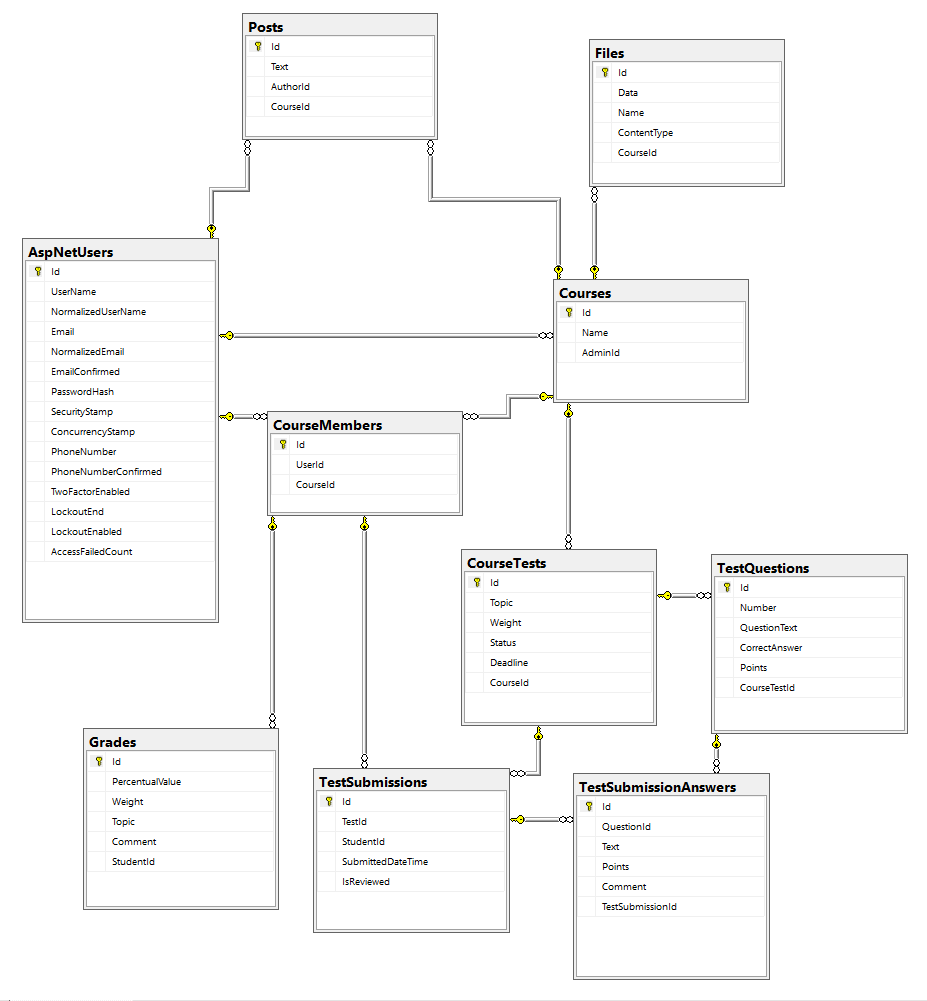
\includegraphics[width=\textwidth]{db_model.PNG}
	\caption{Databázový model aplikace}
\end{figure}

\newpage

např. kód třídy Course vypadá takto:

\begin{lstlisting}
public class Course : IGuidIdObject
{
	public Course()
	{
		Members = new List<CourseMember>();
		Files = new List<CourseFile>();
		Tests = new List<CourseTest>();
		ForumPosts = new List<ForumPost>();
	}
	
	public Course(string name, Person admin) : this()
	{
		Name = name;
		Admin = admin;
	}
	
	/// <summary>
	/// identifier of the couse
	/// </summary>
	[DatabaseGenerated(DatabaseGeneratedOption.Identity)]
	[Key]
	public Guid Id { get; set; }
	
	/// <summary>
	/// name of the course
	/// </summary>
	[Required]
	public string Name { get; set; }
	
	...
\end{lstlisting}

Vidíme, že každá entita obsahuje veřejné vlastnosti (public properties) s gettery a settery. Tyto vlastnosti budou v databázové tabulce reprezentovány jako sloupce. Některé z nich (jako např. Id) obsahují ještě doplňující atributy, ty slouží k upřesnění informací o dané vlastnosti. Například atribut [Key] určuje, že tato vlastnost bude v databázi primární klíč, atribut [Required] určuje, že daný sloupec bude v tabulce u všech záznamů povinný (tedy hodnoty budou NOT NULL).
Dále musí každá entita obsahovat konstruktor bez parametrů.

Vazby mezi entitami jsou reprezentované pomocí tzv. navigačních vlastností. V případě, že chceme vytvořit vazbu typu one-to-many mezi entitami A a B, stačí do vlastností třídy A přidat kolekci objektů typu B, a naopak do třídy B vlastnost typu A. Framework pak při provádění migrace vytvoří v databázové tabulce entity B vytvoří sloupec s cizím klíčem, který bude obsahovat identifikátor entity A, ke které patří.

V aplikaci je vazba one-to-many použita mimo jiné mezi entitami Course a CourseTest, a to tak, že každý test je obsažen v právě jednom kurzu, a v daném kurzu může být N testů.
Kód pak tedy vypadá takto: ve třídě Course je kolekce objektů typu CourseTest

\begin{lstlisting}
/// <summary>
/// tests in this course
/// </summary>
public ICollection<CourseTest> Tests { get; set; }
\end{lstlisting}

a ve třídě CourseTest je pak vlastnost typu Course

\begin{lstlisting}
/// <summary>
/// course that contains this test
/// </summary>
[Required]
public Course Course { get; set; }
\end{lstlisting}

Po provedení databázové migrace (viz. dále) se v tabulce CourseTest vytvoří sloupec CourseId s cizím klíčem, který odkazuje na identifikátor kurzu (tzn. vlastnost Course.Id).

Také si můžeme všimnout, že všechny entity (kromě entity Person) implementují rozhraní IGuidObject. To je jednoduché rozhraní, které obsahuje pouze jednu vlastnost - Id typu Guid. Tímto máme zajištěnou jednotu identifikátorů, tedy že všechny entity, které toto rozhraní implementují, budou mít identifikátor typu Guid.

\begin{lstlisting}
/// <summary>
/// interface for object with <see cref="Guid"/> identifier
/// </summary>
public interface IGuidIdObject
{
	/// <summary>
	/// identifier of the object
	/// </summary>
	Guid Id { get; set; }
}
\end{lstlisting}


Typ Guid jsme zvolili hlavně z toho důvodu, že vestavěné tabulky frameworku (např. Identity) mají také řetězcové identifikátory. Navíc se pak zjednoduší práce ve frontend části (není potřeba parsovat string na int např. v klientské části při práci s URL). Tyto identifikátory generuje databáze, takže je zajištěno, že jsou unikátní.
Další možnost by byla použít jako identifikátor číslo (např. typ int), ale vzhledem k výše uvedeným argumentům je typ Guid v tomto případě lepší možnost.

Dále se v projektu nachází také rozhraní ICourseReferenceObject a ICourseMemberReferenceObject, které slouží k tomu, abychom mohli dále v aplikaci jednotně pracovat s objekty, které mají referenci na entitu Course, resp. CourseMember. Tyto rozhraní implementují pouze nějaké entity.

V programu je dále třída CMSDbContext, která reprezentuje databázový kontext této aplikace. Každý objekt typu DbSet pak představuje jednu databázovou tabulku. Ve třídě je CMSDbContext tedy kolekce typu DbSet pro každou z entit.

\begin{lstlisting}
public DbSet<Grade> Grades { get; set; }

public DbSet<Course> Courses { get; set; }

...
\end{lstlisting}

Jediná výjimka je entita Person, která dědí ze třídy IdentityUser, a jejíž DbSet je nakonfigurovaný ve frameworku. 

V programu pak dále používáme ke komunikaci s databází pouze třídu CMSDbContext a objekty typu DbSet. Třida DbSet<TEntity> implementuje rozhraní IQueryable<TEntity>, takže na ní lze použít LINQ. Takže pokud bych chtěl například vybrat všechny kurzy, jejiž jméno začíná na písmeno C, pak stačí použít následující LINQ dotaz
\begin{lstlisting}
dbContext.Courses.Where(course => course.Name.StartsWith("C"))
\end{lstlisting}
kde proměnná dbContext je instance třídy CMSDbContext.

Ve třídě CMSDbContext je také metoda ConfigureForeignKeys, která provede konfiguraci cizích klíčů v aplikaci. Všechny políčka s cizími klíči jsou v databázi povinné (tzn. NOT NULL), to je zajištěno pomocí atributu [Required] daných vlastností. Nastavením DeleteBehavior.Restrict u cizích klíčů zajistíme, že databáze zůstane v konzistentním stavu. Pokud bychom tedy chtěli smazat entitu, pak na ní nesmí pomocí cizích klíčů odkazovat jiné entity. V opačném případě program při zavolání metody SaveChanges() na databázovém kontextu vyhodí výjimku.

V programu je dále složka Migrations. Při vývoji byl použit princip Code first, tedy že v kódu specifikujeme entity pomocí klasických tříd. Framework se pak postará o vytvoření databázových tabulek z tohoto kódu.

Pokud jsem tedy nějak změníme některou z entit (to může být např. přidání vlastnosti, změna jména vlastnosti, apod.), pak pomocí ORM můžeme vygenerovat soubor popisující tzv. databázovou migraci, která slouží k aplikaci změn z kódu do databáze. Ke každé migraci se vygeneruje jeden soubor, který obsahuje popis změn, které se později provedou v databázi.

K vytváření migrací jsem použijeme nástroj CLI tools for Entity Framework Core. https://docs.microsoft.com/cs-cz/ef/core/cli/dotnet. Pro vygenerování migrace ze změn v kódu použijeme příkaz:

TO-Do: přesunout přesný příkaz jinam

\begin{lstlisting}
dotnet ef migrations add {migration_name} 
--project CourseManagementSystem.Data 
--startup-project CourseManagementSystem.API
\end{lstlisting}

Tímto se vytvoří soubor popisující změny v migraci, ale databáze zatím zůstala beze změny. Tento soubor obsahuje třídu, jenž dědí ze třídy Migration a obsahuje metody Up a Down. V metodě Up je popis změn, které se provedou při aplikaci této migrace, naopak v metodě Down je popis změn, které se provedou v případě odstranění migrace.

Jako příklad si můžeme představit migraci, která obsahuje přidání vlastnosti ScoreWeight k entitě CourseTest (tato vlastnost popisuje váhu testu).
Vygenerovaný kód migrace vypadá takto:

\begin{lstlisting}
public partial class TestWeight_added : Migration
{
	protected override void Up(MigrationBuilder migrationBuilder)
	{
		migrationBuilder.AddColumn<int>(
		name: "ScoreWeight",
		table: "CourseTests",
		nullable: false,
		defaultValue: 0);
	}
	
	protected override void Down(MigrationBuilder migrationBuilder)
	{
		migrationBuilder.DropColumn(
		name: "ScoreWeight",
		table: "CourseTests");
	}
}
\end{lstlisting}

TO-DO: přesunout syntaxi příkaz jinam

Pro promítnutí změn do databáze následně použijeme příkaz:

\begin{lstlisting}
dotnet ef database update 
--project CourseManagementSystem.Data 
--startup-project CourseManagementSystem.API
\end{lstlisting}

Tímto tedy dojde k změnám v databázi (v našem příkladu se vytvoří sloupec ScoreWeight v tabulce CourseTests).

V obou příkazech je potřeba specifikovat cílový a startup projekt. Cílový projekt je ten, který obsahuje databázový kontext a entity naší aplikace (v tomto případě projekt Data). Naopak startup projekt je projekt, který je spouštěný frameworkem, což je potřeba pro získání konfiguračních informací o projektu, jako je například connection string do naší databáze.

\newpage

\subsection{Services}
V tomto projektu se nachází pomocné služby pro komunikaci s databází. 

Jako základ pro všechny služby slouží abstraktní třída DbService, která obsahuje referenci na databázový kontext aplikace a jedinou metodu CommitChanges(). Ta slouží k uložení změn provedených v databázovém kontextu do databáze. 

To je potřeba, protože k uložení změn do databáze dojde až tehdy, když na databázovém kontextu zavoláme metodu SaveChanges(). Pokud bychom tedy například do databázového kontextu něco uložili (např. takto: 
\begin{lstlisting}
dbContext.Grades.Add(new Grade())
\end{lstlisting}
a nezavolali metodu dbContext.SaveChanges(), data by se neuložila.

\begin{lstlisting}
/// <summary>
/// class representing base database service
/// </summary>
public abstract class DbService : IDbService
{
	/// <summary>
	/// context of the CMS database
	/// </summary>
	protected readonly CMSDbContext dbContext;
	
	/// <summary>
	/// construct a new database service
	/// </summary>
	/// <param name="dbContext">CMS database context</param>
	protected DbService(CMSDbContext dbContext)
	{
		this.dbContext = dbContext;
	}
	
	/// <inheritdoc/>
	public void CommitChanges()
	{
		dbContext.SaveChanges();
	}
}
\end{lstlisting}

Tato třída implementuje rozhraní IDbService, které obsahuje pouze metodu CommitChanges().

Dále jsou ve složce Interfaces rozhraní pro další služby, ty jsou rozdělené podle entit (typicky máme pro jednu entitu jednu službu). Všechny tyto rozhraní také implementují rozhraní IDbService. 

Například rozhraní ICourseService (slouží pro práci s kurzy) vypadá takto:
\begin{lstlisting}
public interface ICourseService : IDbService
{
	/// <summary>
	/// get course by its id
	/// </summary>
	/// <param name="courseId">identifier of the course</param>
	/// <returns></returns>
	Course GetById(string courseId);
	
	/// <summary>
	/// archive course by its id
	/// </summary>
	/// <param name="courseId">id of the course to delete</param>
	void ArchiveById(string courseId);
	
	/// <summary>
	/// add the course into the database
	/// </summary>
	/// <param name="course">course to add</param>
	void AddCourse(Course course);
	...
\end{lstlisting}

Ve složce Implementations jsou potom implementace těchto rozhraní. Můžeme vidět, že všechny implementace dědí ze třídy DbService, a zároveň také tranzitivně implementují IDbService.

Například třída CourseService, která implementuje rozhraní ICourseService vypadá takto:

\begin{lstlisting}
public class CourseService : DbService, ICourseService
{
	public CourseService(CMSDbContext dbContext) : base(dbContext)
	{ }
	
	/// <inheritdoc/>
	public void ArchiveById(string courseId)
	{
		Course c = GetById(courseId);
		c.IsArchived = true;
	}
	
	/// <inheritdoc/>
	public Course GetById(string courseId)
	{
		return dbContext.Courses.FindById(courseId);
	}
	
	/// <inheritdoc/>
	public void AddCourse(Course course)
	{
		dbContext.Courses.Add(course);
	}
	...
\end{lstlisting}

Vidíme, že služby typicky pracují s databázovým kontextem, a s daty (vyhledávání, mazání, apod.).
Dále si můžeme všimnout, že v žádné metodě se neukládájí změny do databáze (tzn. volání metody CommitChanges()). To je z toho důvodu, že ve vyšších vrstvách aplikace (např. API) v jedné metodě často voláme několik služeb, příp. několik metod z jedné služby. 
Pokud bychom v metodách služeb přímo ukládali změny do databáze (metoda CommitChanges()), pak bychom se mohli lehce dostat to nekonzistentního stavu. To například tak, že při volání několika služeb v rámci jedné metody by 
mohla některá ze služeb vyhodit výjimku, nicméně všechny služby zavolané předtím by už data uložily.

Takže je na zodpovědnosti volajícího provést uložení změn do databáze, tedy zavolat metodu CommitChanges(), což je typicky poslední příkaz v dané metodě.
Tím jsme tedy zajistili konzistenci dat - buď se do databáze uloží všechny změny provedené v databázovém kontextu, nebo žádné.

Dále si můžeme všimnout, že ve službách pracujeme s identifikátory typu string, ale v databázi používáme typ Guid. To je z toho důvodu, že ve vyšších vrstvách aplikace se pohodlněji pracuje se stringy (např. často dostáváme ID jako URL parametr). Převod mezi typy string a Guid pak řešíme ve službách.

Ve složce Extensions jsou pak pomocné extension metody pro práci s některými třídami.

Ve třídě DbSetExtensions se nachází extension metody pro třídu DbSet<T>. Vybereme si například metodu GetCourseIdOf, ta slouží k získání ID kurzu, ke kterému daný objekt, jenž má referenci na entitu Course, patří.
\begin{lstlisting}
/// <summary>
/// get id of <see cref="Data.Models.Course"/> that the object belongs to
/// </summary>
/// <typeparam name="T">type of items</typeparam>
/// <param name="dbSet">database set</param>
/// <param name="objectId">identifier of the object we look for in <paramref name="dbSet"/></param>
/// <returns></returns>
public static string GetCourseIdOf<T>(this DbSet<T> dbSet, string objectId) where T : class, ICourseReferenceObject, IGuidIdObject
{
	return dbSet.Include(item => item.Course)
		.Single(item => item.Id.ToString() == objectId)
		.Course.Id.ToString();
}
\end{lstlisting}

Vidíme, že toto je jeden z příkladů použití rozhraní ICourseReferenceObject, které se nachází v projektu Data.

V projektu též máme rozhraní ICourseReferenceService, to implementují všechny služby, jejichž entity logicky patří k nějakému kurzu. Rozhraní obsahuje jedinou metodu GetCourseIdOf(string objectId), která získá ID kurzu, ke kterému daná entita patří. V implementaci této metodu pak typicky používáme extension metodu GetCourseIdOf pro třídu DbSet<T>. Například ve třídě CourseTestService vypadá implementace takto:

\begin{lstlisting}
public string GetCourseIdOf(string objectId)
{
	return dbContext.CourseTests.GetCourseIdOf(objectId);
}
\end{lstlisting}

Podobně je v projektu i rozhraní ICourseMemberReferenceService, které používají služby, jejichž entity mají referenci na třídu CourseMember.

Použitím služeb jsme odstranili duplikátní kód (např. hledání kurzu podle ID se používá na několika místech ve vyšších vrstvách), a extrahovali některé složitější dotazy do samostatných metod. To je výhodné hlavně z toho důvodu, že je pak můžeme nezávisle otestovat. Další výhoda je, že vyšší vrstvy jsou odstíněny od použití ORM (a databázového kontextu), pouze volají tyto služby.

Dále si můžeme všimnout, že ve službách používáme při komunikaci s databázovým kontextem tzv. Eager loading (pomocí metod Include()). To znamená, že data databázových entit které daná entita referencuje, se při výchozím chování nenačtou (pokud nepoužijeme metodu Include), tzn. budou mít hodnotu NULL.

Například pro získání testu s otázkami můžeme použít tento příkaz:
\begin{lstlisting}
dbContext.CourseTests
	.Include(test => test.Questions)
\end{lstlisting}
Pokud bych volání metody Include() vynechal, tak by se data otázek nenačetla.

\newpage

\subsection{API}
V tomto projektu se nachází API, které slouží pro komunikaci klientské části se serverovou.

\subsubsection*{Controllers}
Controllery slouží primárně ke zpracování HTTP požadavků. Vidíme, že Controller je klasická C\# třída, jenž dědí ze třídy ControllerBase. Ve většině případů obsahuje reference na služby (jako privátní položky).

\begin{lstlisting}
[Route("api/[controller]")]
[ApiController]
[Authorize]
public class CoursesController : ControllerBase
{
	private readonly IHttpContextAccessor httpContextAccessor;
	private readonly ICourseService courseService;
	private readonly IPeopleService peopleService;
	private CourseTestFilter courseTestFilter;
	
	public CoursesController(IHttpContextAccessor httpContextAccessor, ICourseService courseService, IPeopleService peopleService)
	{
		this.httpContextAccessor = httpContextAccessor;
		this.courseService = courseService;
		this.peopleService = peopleService;
		courseTestFilter = new CourseTestFilter();
	}
	...
\end{lstlisting}

Jednotlivé Controllery pak obsahují veřejné metody, jenž odpovídají HTTP endpointům.

Například následující metoda slouží k získaní všech členů daného kurzu.
\begin{lstlisting}
/// <summary>
/// get all course members
/// </summary>
/// <param name="id">Id of the course</param>
[HttpGet("{id}/members")]
[AuthorizeCourseAdminOf(EntityType.Course, "id")]
public IEnumerable<CourseMemberOrAdminVM> GetAllMembers(string id)
{
	var people = courseService.GetMembersWithUsers(id);
	return people.Select(cm => new CourseMemberOrAdminVM(cm.Id.ToString(), cm.User.UserName, cm.User.Email));
}
\end{lstlisting}

Vidíme, že je tedy označená atributem HttpGet, který zároveň obsahuje URL, přes kterou lze tuto metodu zavolat. V tomto případě je URL suffix "\{id\}/members". Položka Id označuje parametr, jenž má stejnou hodnotu jako proměnná id (parametr metody). Tento suffix se připojí za URL daného Controlleru, a tím získáme celou URL k zavolání této metody. V našem případě dostaneme
\newline
"http://host/api/courses/course-id/members", kde course-id je identifikátor příslušného kurzu a host označuje URL serveru, na kterém aplikace běží. Pokud máme aplikaci spuštěnou lokálně, pak by hodnota měla být localhost:5001. Při HTTP GET dotazu na tuto URL by tedy aplikace zavolala tuto metodu, a vrátila data.

Metoda dále obsahuje atribut určený k autorizaci, pomocí něhož ověříme, že klient má dostatečná práva. V tomto případě povolíme zavolat metodu pouze administrátorům daného kurzu.

V těle metody pak zavoláme konkrétní službu, která typicky pracuje s databází. Tato služba nám vrátí data (v tomto případě všechny členy daného kurzu), které potom namapujeme na objekty typu ViewModel, a ty vrátíme.

\vspace{\baselineskip}

V dalším příkladu máme metodu, která slouží k vytvoření nového kurzu.
\begin{lstlisting}
/// <summary>
/// create new course
/// </summary>
[HttpPost("create")]
public void Create(AddCourseVM courseVM)
{
	string currentUserId = httpContextAccessor.HttpContext.GetCurrentUserId();
	Person admin = peopleService.GetById(currentUserId);
	Course createdCourse = new Course(courseVM.Name, admin);
	
	courseService.AddCourse(createdCourse);
	
	courseService.CommitChanges();
}
\end{lstlisting}
Tato metoda je označena atributem HttpPost, který opět obsahuje URL suffix. Pokud bychom tedy chtěli zavolat tuto metodu, pak je potřeba provést HTTP POST požadavek na URL
\newline
"http://host/api/courses/create", který v těle obsahuje JSON objekt typu AddCourseVM. Framework pak provede deserializaci objektu, a objekt (instanci třídy AddCourseVM) předá jako parametr do této metody.

V těle metody následně vytvoříme nový objekt kurzu, a pomocí příslušné služby (v tomto případě CourseService) jej přidáme k existujícím kurzům. Můžeme si všimnout, že na konci metody voláme metodu CommitChanges(), která změny zapíše do databáze.

\subsubsection*{ViewModels}

ViewModels reprezentují objekty pro komunikaci mezi Frontend a Backend částí (konkrétně mezi Frontend službami a API). Tedy např. při GET dotazu vrací příslušný Controller objekt (příp. objekty) typu ViewModel. Stejně tak při POST dotazu posílá klient v těle požadavku objekt typu ViewModel.

Příklad:
\begin{lstlisting}
/// <summary>
/// viewmodel for submitting a test
/// </summary>
public class SubmitTestVM
{
	public SubmitTestVM()
	{
	}
	
	public SubmitTestVM(string testId, string testTopic, bool isSubmitted, IEnumerable<SubmissionAnswerVM> answers, bool isTestGraded)
	{
		TestSubmissionId = testId;
		TestTopic = testTopic;
		Answers = answers;
		IsSubmitted = isSubmitted;
		IsTestGraded = isTestGraded;
	}
	
	/// <summary>
	/// id of the test submission
	/// </summary>
	[RequiredWithDefaultErrorMessage]
	public string TestSubmissionId { get; set; }
	
	/// <summary>
	/// topic of the test
	/// </summary>
	[RequiredWithDefaultErrorMessage]
	public string TestTopic { get; set; }
	
	/// <summary>
	/// check if the test has already been submitted
	/// </summary>
	public bool IsSubmitted { get; set; }
	...
\end{lstlisting}

Tento ViewModel reprezentuje data odevzdávaného testu. Vidíme, že ViewModely jsou typicky veřejné třídy s veřejnými vlastnostmi. Dále vidíme, že ViewModel má veřejný bezparametrový konstuktor, ten je volán při deserializaci dat.

Také si můžeme všimnout, že u některé vlastnosti ještě obsahují doplňující atributy (např. atribut [RequiredWithDefaultErrorMessage] u vlastnosti TestTopic). Tyto atributy slouží primárně k validaci dat.

Ve ViewModelech poměrně často používáme dědičnost, podobně jako v tomto příkladu.
\begin{lstlisting}
/// <summary>
/// base viewmodel for course tests
/// </summary>
public abstract class BaseCourseTestVM
{
	protected BaseCourseTestVM()
	{
	}
	
	protected BaseCourseTestVM(int weight, string topic, ...)
	{
		...
	}
	
	/// <summary>
	/// weight of the score from the test (e.g. test of weight 2 has twice bigger impact on overall score than test of weight 1)
	/// </summary>
	[PositiveIntValue]
	public int Weight { get; set; }
	
	/// <summary>
	/// topic of the test
	/// </summary>
	[RequiredWithDefaultErrorMessage]
	public string Topic { get; set; }

	...
}

/// <summary>
/// viewmodel for adding a course test
/// </summary>
public class AddCourseTestVM : BaseCourseTestVM
{
	public AddCourseTestVM() : base()
	{ }
}

/// <summary>
/// viewmodel representing a test in a course
/// </summary>
public class CourseTestDetailsVM : BaseCourseTestVM
{
	public CourseTestDetailsVM() : base()
	{ }
	
	public CourseTestDetailsVM(string id, string topic, int scoreWeight, ...)
	: base(scoreWeight, topic, ...)
	{
		Id = id;
		Status = testStatus;
	}
	
	/// <summary>
	/// id of the test
	/// </summary>
	[RequiredWithDefaultErrorMessage]
	public string Id { get; set; }
	
	/// <summary>
	/// status of the test
	/// </summary>
	public TestStatus Status { get; set; }
}
\end{lstlisting}
Chceme vytvořit alespoň dva ViewModely, jejichž struktura je velmi podobná a liší se jen přítomností několika málo doplňujících vlastností. Řešením je vytvořit Base třídu, která obsahuje všechny společné vlastnosti. Pro konkrétní ViewModely poté můžeme vytvořit třídy, které dědí z této rodičovské třídy, a obsahují již pouze doplňující vlastnosti.

Ve výše uvedeném příkladu máme tedy třídu BaseCourseTestVM, a od ní dědí třídy AddCourseTestVM a CourseTestDetailsVM. Tyto ViewModely slouží k přidání nového testu, resp. získání informací o daném testu.

Vidíme, že vlastnosti Id a Status se nachází pouze ve třídě CourseTestDetailsVM. Toto dává smysl, jelikož při vytváření testu ještě neznáme jeho identifikátor (objekt ještě není uložený v databázi).
Podobně je to i se stavem (vlastnost Status), jelikož ten bude při vytváření vždy nastaven na New.

Bylo by samozřejmě možné oba ViewModely sloučit do jedné třídy se všemi vlastnostmi. Toto řešení je ale podle mého názoru velmi matoucí, jelikož vlastnosti Id a Status jsou při vytváření testu zbytečné.

\subsubsection*{Atributy určené k validaci}

V programu používáme několik vlastních atributů, určených k validaci dat, ty se nachází ve složce Validation/Attributes.
Atribut je klasická C\# třída, která dědí ze třídy System.Attribute. Její název obvykle končí suffixem "Attribute".

Příklady:
\begin{lstlisting}
/// <summary>
/// Validation attribute that marks this value as required
/// <br/>
/// if validation fails <see cref="defaultErrorMessage"/> is displayed
/// </summary>
public class RequiredWithDefaultErrorMessageAttribute : RequiredAttribute
{
	/// <summary>
	/// default error message displayed ({0} is replaced by the field name that this attribute belongs to)
	/// </summary>
	public const string defaultErrorMessage = "The field {0} is required";
	
	public RequiredWithDefaultErrorMessageAttribute()
	{
		ErrorMessage = defaultErrorMessage;
	}
}

/// <summary>
/// Validation attribute that validates if the double value is non-negative (e.g. >=0)
/// <br/>
/// if validation fails <see cref="defaultErrorMessage"/> is displayed
/// </summary>
public class NonNegativeDoubleValueAttribute : RangeAttribute
{
	/// <summary>
	/// default error message displayed ({0} is replaced by the field name that this attribute belongs to)
	/// </summary>
	public const string defaultErrorMessage = "The field {0} must be non-negative";
	
	public NonNegativeDoubleValueAttribute() : base(0, double.MaxValue)
	{
		ErrorMessage = defaultErrorMessage;
	}
}
\end{lstlisting}

\begin{itemize}
\item NonNegativeDoubleValueAttribute -- Tento atribut validuje, že vlastnost typu double, ke které patří, je nezáporné číslo. V případě, že tomu tak není, nastavíme výchozí chybovou hlášku "The field \{0\} must be non-negative", kde \{0\} je název vlastnosti, ke které atribut patří.

\item RequiredWithDefaultErrorMessageAttribute -- Tento atribut dědí z atributu RequiredAttribute. Pokud má příslušná vlastnost hodnotu null, nebo se jedná o řetězec, který je prázdný, nebo složený pouze z bílých znaků, tak validace selže. Atribut RequiredWithDefaultErrorMessage pak slouží jen k přidání výchozí chybové hlášky "The field \{0\} is required", v případě, že validace selže.

\end{itemize}

Dále jsou v aplikaci ještě použité atributy NonNegativeIntValueAttribute a PositiveIntValueAttribute.


\subsubsection*{Error Handling}

V případě, že nastane chyba při deserializaci dat (např. klient pošle v těle POST dotazu nevalidní data), tak framework vyhodí výjimku a vrátí objekt, který popisuje chybu. \url{https://docs.microsoft.com/en-us/aspnet/core/web-api/?view=aspnetcore-5.0#automatic-http-400-responses}

Pokud nastane chyba při obsluze dotazu (např. klient se pomocí GET dotazu pokusí získat informace o nějaké již smazané entitě), pak v programu vyhodíme výjimku. Všechny výjimky jsou pak zachyceny třídou ErrorHandlerController, která funguje jako obecný Error handler.
Toto je nakonfigurováno v metodě Configure(), jenž se nachází ve třídě Startup.
\begin{lstlisting}
/// <summary>
/// controller for error handling
/// </summary>
[ApiExplorerSettings(IgnoreApi = true)]
public class ErrorHandlerController : ControllerBase
{
	private const string generalErrorText = "An error occurred while processing the request.";
	
	/// <summary>
	/// handle runtime error
	/// </summary>
	/// <returns></returns>
	[Route("errorHandler")]
	public IActionResult HandleError()
	{
		var context = HttpContext.Features.Get<IExceptionHandlerFeature>();
		var exception = context.Error; // thrown exception
		
		var errorDescription = new Dictionary<string, string[]>
		{
			{ "Request failed", new string[] { generalErrorText } }
		};
		
		var errorsVM = new ErrorsDictionaryVM(errorDescription);
		return BadRequest(errorsVM);
	}
}
\end{lstlisting}
Metoda HandleError tedy nastaví kód odpovědi na 400 Bad Request, a vrátí objekt typu ErrorsDictionaryVM.
Ten v tomto případě obsahuje obecnou hlášku "An error occurred while processing the request."

\subsubsection*{Autorizace}

V programu máme také server-side autorizaci. Ta slouží k ověření toho, jestli je uživatel oprávněný provést danou akci. Základní entitou pro autorizaci je kurz (entita Course). V aplikaci tedy vždy ověřujeme, jestli je aktuální uživatel administrátor (příp. člen) kurzu, ke kterému se vztahuje daná entita (např. CourseTest).

K tomuto účelu používáme autorizační atributy, které se nachází ve složce Auth/Attributes. 
Abstraktní třída CourseBasedAuthorizeFilter slouží jako rodičovská třída pro všechny filtry, založené na autorizaci pomocí kurzů.

\begin{lstlisting}
/// <summary>
/// filter for authorization based on <see cref="Data.Models.Course"/> related entity
/// </summary>
public abstract class CourseBasedAuthorizeFilter : IAuthorizationFilter
{
	/// <summary>
	/// type of the course related entity
	/// </summary>
	private readonly EntityType entityType;
	
	/// <summary>
	/// name of the field in HTTP route that contains the id of the entity
	/// </summary>
	private readonly string entityIdFieldName;
	
	/// <summary>
	/// factory for <see cref="Services.Interfaces.ICourseReferenceService"/> services
	/// </summary>
	private readonly ICourseReferenceServiceFactory courseReferenceServiceFactory;

	/// <inheritdoc/>
	public void OnAuthorization(AuthorizationFilterContext context)
	{
		if (context.HttpContext.User.Identity.IsAuthenticated)
		{
			string currentUserId = context.HttpContext.GetCurrentUserId();
			string objectId = context.HttpContext.Request
				.RouteValues[entityIdFieldName].ToString();
			
			var service = courseReferenceServiceFactory
				.GetByEntityType(entityType);
			string courseId = service.GetCourseIdOf(objectId);
			
			if (IsAuthorized(currentUserId, courseId, entityType, objectId))
			{
				// authorization passed -> proceed to controller
				return;
			}			
		}
		context.Result = new UnauthorizedResult();
	}
	
	/// <summary>
	/// check if the user is authorized to access the course related entity
	/// </summary>
	/// ...
	protected abstract bool IsAuthorized(string currentUserId, string courseId, EntityType entityType, string entityId);
	
	...
}
\end{lstlisting}

Vidíme, že tato třída obsahuje typ entity (proměnná entityType), pomocí které provádíme autorizaci. Dále také název proměnné v URL, která obsahuje identifikátor této entity. 

Metoda OnAuthorization se automaticky zavolá při autorizaci. V této metodě nejprve zkontrolujeme, že uživatel je přihlášený, poté získáme jeho ID (přes HttpContext) a ID dané entity. Poté získáme identifikátor kurzu, ke kterému daná entita logicky patří. Zde využíváme toho, že všechny služby implementují rozhraní ICourseReferenceService. 
Dále zjistíme, jestli má uživatel dostatečná práva. K tomuto účelu slouží abstraktní metoda IsAuthorized. 

Jedná se o využití návrhového vzoru Template method, kdy implementaci této metody necháme na třídách, které dědí z CourseBasedAuthorizeFilter. 
Společné kroky autorizace nicméně implementujeme v této (rodičovské) třídě.

Pokud zjistíme, že uživatel nemá dostatečná práva, pak pouze vrátíme UnauthorizedResult, a požadovaná akce se neprovede.

Dále ještě potřebujeme v aplikaci mechanismus, který nám podle enumu EntityType vrátí příslušnou službu. K tomuto účelu používáme třídu CourseReferenceServiceFactory.
\begin{lstlisting}
/// <summary>
/// factory for <see cref="ICourseReferenceService"/>
/// </summary>
public class CourseReferenceServiceFactory : ICourseReferenceServiceFactory
{
	...
	
	private readonly IReadOnlyDictionary<EntityType, ICourseReferenceService> dataServices;
	
	public CourseReferenceServiceFactory(ICourseAdminService courseAdminService, ICourseMemberService courseMemberService, ...)
	{
		dataServices = new Dictionary<EntityType, ICourseReferenceService>
		{
			[EntityType.CourseMember] = courseMemberService,
			[EntityType.CourseAdmin] = courseAdminService,
			[EntityType.CourseTest] = courseTestService,
			...
		};
	}
	
	/// <inheritdoc/>
	public ICourseReferenceService GetByEntityType(EntityType entityType)
	{
		return dataServices[entityType];
	}
}
\end{lstlisting}

Tato třída obsahuje slovník dataServices, ve kterém je pod daným klíčem typu EntityType uložená příslušná služba.
V metodě GetByEntityType pak jen vrátíme položku ze slovníku.
Opět využíváme toho, že všechny služby implementují rozhraní ICourseReferenceService.

V aplikaci používáme tyto autorizační filtry (všechny dědí ze třídyCourseBasedAuthorizeFilter).
\begin{itemize}
	\item CourseAdminAuthorizeFilter -- ověřuje, jestli je aktuální uživatel administrátor kurzu, ke kterému patří daná entita. Používáme v akcích, které může provádět pouze admin daného kurzu (jako např. vytváření nových testů).
	\item CourseAdminOrMemberAuthorizeFilter -- ověřuje, zda je aktuální uživatel administrátor nebo člen kurzu, ke kterému patří daná entita. Tento filtr používáme např. v metodě pro získání všech souborů v daném kurzu.
	\item CourseAdminOrOwnerAuthorizeFilter -- podobně jako 1. filtr slouží k ověření toho, jestli je aktuální uživatel administrátor kurzu, k němuž patří daná entita. Zároveň ale akci povolíme provést, pokud je uživatel vlastníkem dané entity. To znamená, že příslušná entita (např. odevzdaný test - entita TestSubmission) se váže k danému uživateli. Toto ověření používáme například v metodě pro získání opraveného testu.
\end{itemize}

Například třída CourseAdminOrMemberAuthorizeFilter vypadá takto:
\begin{lstlisting}
public class CourseAdminOrMemberAuthorizeFilter : CourseBasedAuthorizeFilter
{
	private readonly IPeopleService peopleService;
	
	/// <inheritdoc/>
	protected override bool IsAuthorized(string currentUserId, string courseId, EntityType entityType, string objectId)
	{
		return peopleService.IsAdminOfCourse(currentUserId, courseId) || peopleService.IsMemberOfCourse(currentUserId, courseId);
	}
	...
}
\end{lstlisting}

Ke každému autorizačnímu filtru se pak vztahuje atribut.
\begin{lstlisting}
public class AuthorizeCourseAdminOrMemberOfAttribute : TypeFilterAttribute
{
	public AuthorizeCourseAdminOrMemberOfAttribute(EntityType entityType, string entityIdFieldName) : base(typeof(CourseAdminOrMemberAuthorizeFilter))
	{
		Arguments = new object[] { entityType, entityIdFieldName };
	}
}
\end{lstlisting}

Vidíme, že tento atribut má konstruktor se 2 parametry, které následně předá autorizačnímu filtru. 

Atributy se poté používají následujícím způsobem (v příkladu je atribut použitý na metodě Controlleru, která slouží ke stažení souboru podle daného id).
\begin{lstlisting}
[HttpGet("{id}")]
[AuthorizeCourseAdminOrMemberOf(EntityType.CourseFile, "id")]
public IActionResult Download(string id)
{
	...
}
\end{lstlisting}

Tímto způsobem tedy zaručíme, že k této metodě mají přístup pouze administrátoři a členové daného kurzu, ve kterém je tento soubor sdílen. Pomocí parametrů atributu popíšeme, že entita je soubor, a její identifikátor se nachází v proměnné s názvem id (což je parametr metody).

\subsubsection*{Dependency Injection}

K předávání závislostí v aplikaci používáme mechanismus Dependency injection. 

Používáme vestavěný IoC kontejner ve frameworku ASP .NET Core, konfigurace se nachází ve třídě Startup v metodě ConfigureServices.
U každé závislosti uvedeme její rozhraní a implementaci. 
Závislosti vkládáme do kontejneru ve většině případů pomocí metody AddTransient. To znamená, že při každém dotazu na danou službu v kontejneru se vytvoří nová instance.
\begin{lstlisting}
// add dependencies to IoC container
services.AddTransient<ICourseService, CourseService>();
services.AddTransient<IPeopleService, PeopleService>();
services.AddTransient<IGradeService, GradeService>();
...
\end{lstlisting}
Pokud by naše konfigurace vypadala takto, tak bychom do kontejneru vložili 3 závislosti. První z nich má rozhraní ICourseService a implementaci CourseService, u ostatních závislostí je to obdobně.

Pokud tedy chceme, aby do nějaké třídy, jejíž instance jsou vytvářeny frameworkem, byly dosazeny příslušné závislosti (dependencies), použijeme Constructor injection. V konstruktoru dané třídy vytvoříme pro každou požadovanou závislost 1 parametr, který bude mít stejný typ jako rozhraní dané závislosti. Framework se pak postará o dosazení parametrů podle konfigurace IoC kontejneru.

\begin{lstlisting}
public CoursesController(IHttpContextAccessor httpContextAccessor, ICourseService courseService, IPeopleService peopleService)
{
	this.httpContextAccessor = httpContextAccessor;
	this.courseService = courseService;
	this.peopleService = peopleService;
	...
}
\end{lstlisting}
V tomto případě tedy framework ví, že třída má 3 závislosti, které je potřeba vyhledat v kontejneru.
Podle konfigurace poté například do parametru courseService dosadí novou instanci třídy CourseService. 

Dependency injection používáme primárně v Controllerech.
Nevytváříme tedy přímo instance služeb (pomocí operátoru new), naopak si služby vyžádáme přes parametry konstruktoru, a framework se postará o jejich správné dosazení.

Řešení pomocí Dependency injection je flexibilnější, jelikož Controller nezávisí na implementaci dané služby, ale pouze na jejím rozhraní.

\newpage

\subsection{Tests}

obsahuje testy služeb
TODO: dopsat

\newpage

\section{Klientská část}

\lstset{style=typescript}

Klientská část aplikace se nachází ve složce API/ClientApp, a je napsaná v jazyce Typescript s použitím frameworku Angular.
TODO: dopsat

\subsection{Services}

Služby slouží ke komunikaci frontend části s API. Jedna služba typicky odpovídá jednomu Controlleru a jednotlivé metody služby pak slouží k volání metod API. 

Všechny služby dědí z abstraktní třídy ApiService. 

\begin{lstlisting}
/**
* base class for all API services
*/
export abstract class ApiService {

	/**
	* HTTP client
	* @protected
	*/
	protected readonly http: HttpClient;
	
	/**
	* url of the controller to fetch data (ends with /)
	* @protected
	*/
	protected readonly controllerUrl: string;
	
	/**
	* describes how many times to repeat unsuccessful API request
	* @private
	*/
	private readonly retryCount: number = 1;
	
	/**
	* create new ApiService
	* @param http http client
	* @param baseUrl base url of the app
	* @param controllerName name of controller that the service fetches data from
	* @protected
	*/
	protected constructor(http: HttpClient, baseUrl: string, controllerName: string) {
		this.controllerUrl = baseUrl + `api/${controllerName}/`;
		this.http = http;
	}
	
	/**
	* handle failed HTTP response
	* @param response HTTP error response object
	* @private
	*/
	private handleError(response: HttpErrorResponse) {
		const errorObject: ApiErrorResponseVM = response;
		return throwError(errorObject.error);
	}
	
	/**
	* process HTTP response
	*
	* if it succeeds, return it, otherwise retry {@link retryCount}-times, then throw an error
	* @param response observable of the response
	* @private
	*/
	private processResponse<T>(response: Observable<T>): Observable<T> {
		return response.pipe(
			retry(this.retryCount),
			catchError(this.handleError)
		);
	}
	
	/**
	* execute HTTP GET request to the given URL
	* @param actionUrl URL of the action (will be added to {@link controllerUrl})
	* @protected
	* @returns An Observable of the HTTPResponse, with a response body in the requested type
	*/
	protected httpGet<T>(actionUrl: string): Observable<T> {
		return this.processResponse(this.http.get<T>(this.controllerUrl + actionUrl));
	}
	...
}
\end{lstlisting}

Vidíme, že třída obsahuje URL daného Controlleru, a také pomocné metody pro komunikaci s API. Metoda processResponse slouží ke zpracování odpovědi, v případě neúspěchu se pokusí dotaz opakovat. Pokud dotaz opět skončí neúspěchem, pak zavolá metodu pro obsluhu chyb (handleError).

Metodu processResponse pak využíváme například v metodě httpGet, která poté slouží k volání metod API pomocí HTTP GET dotazů. Obdobně třída obsahuje i metody pro jiné typy HTTP požadavků (POST, PUT, DELETE).

Konkrétní služby dědí ze třídy ApiService, a obsahují metody, které typicky slouží k jednomu dotazu na API.

\begin{lstlisting}
export class CourseTestService extends ApiService {
	private static controllerName = 'courseTests';
	
	constructor(http: HttpClient, @Inject('BASE_URL') baseUrl: string) {
		super(http, baseUrl, CourseTestService.controllerName);
	}
	
	/**
	* get test by Id
	* @param testId
	*/
	public getById(testId: string): Observable<CourseTestDetailsVM> {
		return this.httpGet<CourseTestDetailsVM>(testId);
	}
	
	/**
	* add new test to the given course
	* @param testToAdd test to add
	* @param courseId Id of the course
	*/
	public addToCourse(testToAdd: AddCourseTestVM, courseId: string): Observable<{}> {
		return this.httpPost(courseId, testToAdd);
	}
	
	...
}
\end{lstlisting}

Na příkladu vidíme, že služba obsahuje pevně dané URL Controlleru, který volá; a dále několik metod, které volají metody tohoto API Controlleru.
Například metoda getById slouží k získání testu podle jeho identifikátoru. V těle pouze provedeme HTTP GET dotaz, pomocí generického parametru specifikujeme, že vrácený objekt má být typu CourseTestDetailsVM. 
Obdobně je to u metodu addToCourse, která se používá k přidání nového testu do kurzu. Oproti předchozí metodě obsahuje ještě jeden parametr -- testToAdd, který reprezentuje test, jenž bude vytvořen. Tento objekt pak vloží do těla HTTP požadavku, a odešle. 
Můžeme si všimnout, že v tomto případě voláme metodu httpPost bez generického parametru. To je z toho důvodu, že odpověď je prázdná (tzn. neobsahuje žádný ViewModel).

Vidíme, že tělo metod je typicky velmi krátké, ve většině případů se jedná pouze o HTTP dotaz na danou adresu.

Služby fungují asynchronně, tedy nevrací přímo dané objekty, ale generický typ Observable<T>. Zavoláním metody subscribe() na tomto typu se pak počká na vrácení dat, a klient s nimi může pak dále pracovat.

\newpage

\subsection{ViewModels}

V klientské části se také nacházejí ViewModely, které slouží ke komunikaci s API. Tyto objekty přesně odpovídají ViewModelům ze serverové části (tzn. obsahují stejné položky stejných typů).

Na příkladu vidíme ViewModel, který reprezentuje odeslaný test ()
\begin{lstlisting}
/**
* viewmodel for submitting a test
*/
export class SubmitTestVM {
	/**
	* id of the test submission
	*/
	public testSubmissionId: string;
	
	/**
	* topic of the test
	*/
	public testTopic: string;
	
	/**
	* check if the test has already been submitted
	*/
	public isSubmitted: boolean;
	
	...
}
\end{lstlisting}

Pro HTTP GET frontend služby typicky vrací objekty typu ViewModel. Stejně tak při POST dotazu je do těla požadavku vložen objekt typu ViewModel.

\newpage

\subsection{Components}

\begin{lstlisting}
<div class="jumbotron">
	<h3>Students</h3>
	<table class="table table-striped table-responsive">
		<tr>
			<th>Name</th>
			<th>Email</th>
			<th></th>
		</tr>
		<tr *ngFor="let person of students">
			<td>{{person.name}}</td>
			<td>{{person.email}}</td>
			<td><a class="nav-link" routerLink="/students/{{person.id}}">Details</a></td>
		</tr>
	</table>
</div>
\end{lstlisting}

\begin{lstlisting}
@Component({
selector: 'app-student-list',
templateUrl: './student-list.component.html',
styleUrls: ['./student-list.component.css']
})
export class StudentListComponent implements OnInit {
	
	@Input()
	private courseId: string;
	
	/**
	* list of students
	*/
	public students: CourseMemberOrAdminVM[] = [];
	
	private readonly courseService: CourseService;
	
	constructor(roleAuthService: RoleAuthService, courseService: CourseService) {
		this.courseService = courseService;
	}
	
	ngOnInit() {
		this.courseService.getAllMembers(this.courseId).subscribe(result => {
			this.students = result;
		});
	}
}
\end{lstlisting} 

\begin{lstlisting}
<div *ngIf="!isCourseAdmin">
	<button class="btn btn-success" routerLink="/students/{{currentCourseMemberId}}">My Grades</button>
</div>

<app-test-list [courseId]="courseId" [isCourseAdmin]="isCourseAdmin"></app-test-list>
<app-file-list [courseId]="courseId" [isCourseAdmin]="isCourseAdmin"></app-file-list>
<app-student-list *ngIf="isCourseAdmin" [courseId]="courseId"></app-student-list>
<app-admin-list *ngIf="isCourseAdmin" [courseId]="courseId"></app-admin-list>
<app-course-forum [courseId]="courseId" [isCourseAdmin]="isCourseAdmin"></app-course-forum>
\end{lstlisting}

Routing
\begin{lstlisting}
RouterModule.forRoot([
	{path: '', component: HomeComponent, pathMatch: 'full'},
	{path: 'students/:id', component: StudentDetailComponent},
	{path: 'courses', component: CourseListComponent},
	{path: 'courses/:id', component: CourseDetailComponent},
	...
\end{lstlisting}

slouží k zobrazování dat, každá komponenta má 2 části: šablonu a backend

\newpage

\section{Zajímavé problémy}

\subsection{ViewModels x DB entity}

Použil jsem různé objekty pro databázové entity a view-modely.

TODO: pořádně rozepsat + vysvětlit + ukázka kódu

\subsection{ViewModels v serverové i klientské části}

view-modely jsou v serverové i klientské části aplikace

TODO: pořádně rozepsat + vysvětlit + ukázka kódu

\chapter{Uživatelská dokumentace}
Popis všech funkcí + screenshoty?

TODO: rozepsat mnohem více do detailu (krok po kroku + snímky obrazovky)

(převzato ze specifikace ročníkového projektu)

\section{Vytvoření a administrace kurzu}
Uživatelé budou moci vytvářet nové kurzy, administrátoři daného kurzu budou moci přidávat a odebírat členy. Každý uživatel uvidí v aplikaci seznam kurzů, kam je přihlášen.

\section{Vytváření a vyplňování testů}
Administrátoři kurzu budou moci vytvářet testy, které budou žáci vyplňovat. V případě otázek s nabídkou odpovědí systém správnost sám vyhodnotí, otázky s volnou odpovědí budou hodnoceny ručně. Každý uživatel pak v daném kurzu uvidí seznam známek a bude si moci opravený test zobrazit a prohlédnout. Aplikace bude rozlišovat mezi testy a kvízy (kvízy se nebudou hodnotit známkou).

\section{Odevzdávání a hodnocení úkolů}
Uživatelé budou moci prostřednictvím aplikace odevzdávat úkoly, které jim budou poté ohodnoceny.

\section{Správa obsahu kurzu}
Administrátoři kurzu budou moci editovat obsah kurzu (např. přidávat nové materiály, soubory, apod.) 

\section{Fórum k danému kurzu}
U každého kurzu bude k dispozici fórum. 

\section{Vytváření a správa účtů}
Uživatelé si budou moci vytvářet nové účty, správci je budou moci do daného kurzu zapsat.

\include{kap04}

\chapter*{Závěr}
\addcontentsline{toc}{chapter}{Závěr}

V této práci jsem se zaměřil na vývoj webové aplikace pro správu různých typů výukových kurzů.

Oproti alternativám jako jsou např. aplikace Bakaláři a Moodle není výsledná aplikace zaměřená jen na školní kurzy, 
ale můžeme ji snadno použít i pro jiné typy kurzů, jako jsou např. jazykové či zájmové kurzy. 
Každý uživatel si může v aplikaci vytvářet vlastní kurzy.

Aplikace je rozdělená na serverovou a klientskou část, a naprogramovaná s použitím moderních technlologií, 
jako např. frameworky ASP.NET Core a Angular. Kód programu je uložený ve veřejném repozitáři na GitHubu.

Detailní popis funkcionality se nachází v uživatelské dokumentaci \ref{UserDoc}.


%%% Seznam použité literatury
%%% Seznam použité literatury (bibliografie)
%%%
%%% Pro vytváření bibliografie používáme bibTeX. Ten zpracovává
%%% citace v textu (např. makro \cite{...}) a vyhledává k nim literaturu
%%% v souboru literatura.bib.
%%%
%%% Příkaz \bibliographystyle určuje, jakým stylem budou citovány odkazy
%%% v textu. V závorce je název zvoleného souboru .bst. Styly plainnat
%%% a unsrt jsou standardní součástí latexových distribucí. Styl czplainnat
%%% je dodáván s touto šablonou a bibTeX ho hledá v aktuálním adresáři.

% \bibliographystyle{czplainnat}    %% Autor (rok) s českými spojkami
% \bibliographystyle{plainnat}    %% Autor (rok) s anglickými spojkami
\bibliographystyle{unsrt}       %% [číslo]

\renewcommand{\bibname}{Zdroje}

%%% Vytvoření seznamu literatury. Pozor, pokud jste necitovali ani jednu
%%% položku, seznam se automaticky vynechá.

\bibliography{literatura}

%%% Kdybyste chtěli bibliografii vytvářet ručně (bez bibTeXu), lze to udělat
%%% následovně. V takovém případě se řiďte normou ISO 690 a zvyklostmi v oboru.

% \begin{thebibliography}{99}
%
% \bibitem{lamport94}
%   {\sc Lamport,} Leslie.
%   \emph{\LaTeX: A Document Preparation System}.
%   2. vydání.
%   Massachusetts: Addison Wesley, 1994.
%   ISBN 0-201-52983-1.
%
% \end{thebibliography}


%%% Obrázky v bakalářské práci
%%% (pokud jich je malé množství, obvykle není třeba seznam uvádět)
\listoffigures

%%% Použité zkratky v bakalářské práci (opět nemusí být nutné uvádět)
%%% U matematických prací může být lepší přemístit seznam zkratek na začátek práce.
\chapwithtoc{Seznam použitých zkratek}

HTTP
API
IL
ORM
IoC
CLR
OOP
HTML
CSS
CI
SQL

%%% Přílohy k bakalářské práci, existují-li. Každá příloha musí být alespoň jednou
%%% odkazována z vlastního textu práce. Přílohy se číslují.
%%%
%%% Do tištěné verze se spíše hodí přílohy, které lze číst a prohlížet (dodatečné
%%% tabulky a grafy, různé textové doplňky, ukázky výstupů z počítačových programů,
%%% apod.). Do elektronické verze se hodí přílohy, které budou spíše používány
%%% v elektronické podobě než čteny (zdrojové kódy programů, datové soubory,
%%% interaktivní grafy apod.). Elektronické přílohy se nahrávají do SISu a lze
%%% je také do práce vložit na CD/DVD. Povolené formáty souborů specifikuje
%%% opatření rektora č. 72/2017.
\appendix
\chapter{Přílohy}

\section{Uživatelská dokumentace}
Popis všech funkcí + screenshoty?

TODO: rozepsat mnohem více do detailu (krok po kroku + snímky obrazovky)

(převzato ze specifikace ročníkového projektu)

\subsection{Vytvoření a administrace kurzu}
Uživatelé budou moci vytvářet nové kurzy, administrátoři daného kurzu budou moci přidávat a odebírat členy. Každý uživatel uvidí v aplikaci seznam kurzů, kam je přihlášen.

\subsection{Vytváření a vyplňování testů}
Administrátoři kurzu budou moci vytvářet testy, které budou žáci vyplňovat. V případě otázek s nabídkou odpovědí systém správnost sám vyhodnotí, otázky s volnou odpovědí budou hodnoceny ručně. Každý uživatel pak v daném kurzu uvidí seznam známek a bude si moci opravený test zobrazit a prohlédnout. Aplikace bude rozlišovat mezi testy a kvízy (kvízy se nebudou hodnotit známkou).

\subsection{Odevzdávání a hodnocení úkolů}
Uživatelé budou moci prostřednictvím aplikace odevzdávat úkoly, které jim budou poté ohodnoceny.

\subsection{Správa obsahu kurzu}
Administrátoři kurzu budou moci editovat obsah kurzu (např. přidávat nové materiály, soubory, apod.) 

\subsection{Fórum k danému kurzu}
U každého kurzu bude k dispozici fórum. 

\subsection{Vytváření a správa účtů}
Uživatelé si budou moci vytvářet nové účty, správci je budou moci do daného kurzu zapsat.


\openright
\end{document}
